\vspace{1.5pc}
\section[Domain Penelitian]{Domain Penelitian}
\begin{spacing}{1.5}
	Domain penelitian meliputi wilayah Teluk Benggala (BoB) dengan koordinat ($5.5^\circ-24.6^\circ$ N dan $78.2^\circ-96.7^\circ$ E) dan wilayah perairan Aceh, Selat Malaka, dan bagian Laut Cina Selatan dengan koordinat ($-6.22^\circ-6.8^\circ$ N dan $89.1^\circ-106.6^\circ$ E) (lihat Gambar \ref{fig:domain}). Data batimetri untuk domain penelitian diperoleh dari SRTM15+ \href{https://topex.ucsd.edu/pub/archive/srtm15/V1/}{(https://topex.ucsd.edu/)} - kisi elevasi global yang diperbarui pada interval pengambilan sampel spasial 15 arc-second (ukuran piksel $\sim 500 \times 500$ m di ekuator) \shortcite{Tozer2019}. Penelitian ini dilakukan dengan mengkaji variabilitas lapisan vertikal berdasarkan data meteorology dan aplikasinya di beberapa domain penelitian. Pertimbangan domain ini bertujuan untuk melihat keberlakukan secara umum, terhadap teori iklim dan MLD, oleh karena itu perlu diterapkan aplikasi di beberapa tempat seperti: BoB, Perairan Aceh, Selat Malaka, dan Bagian Laut Cina Selatan.
	\begin{figure}[H]
		\centering
		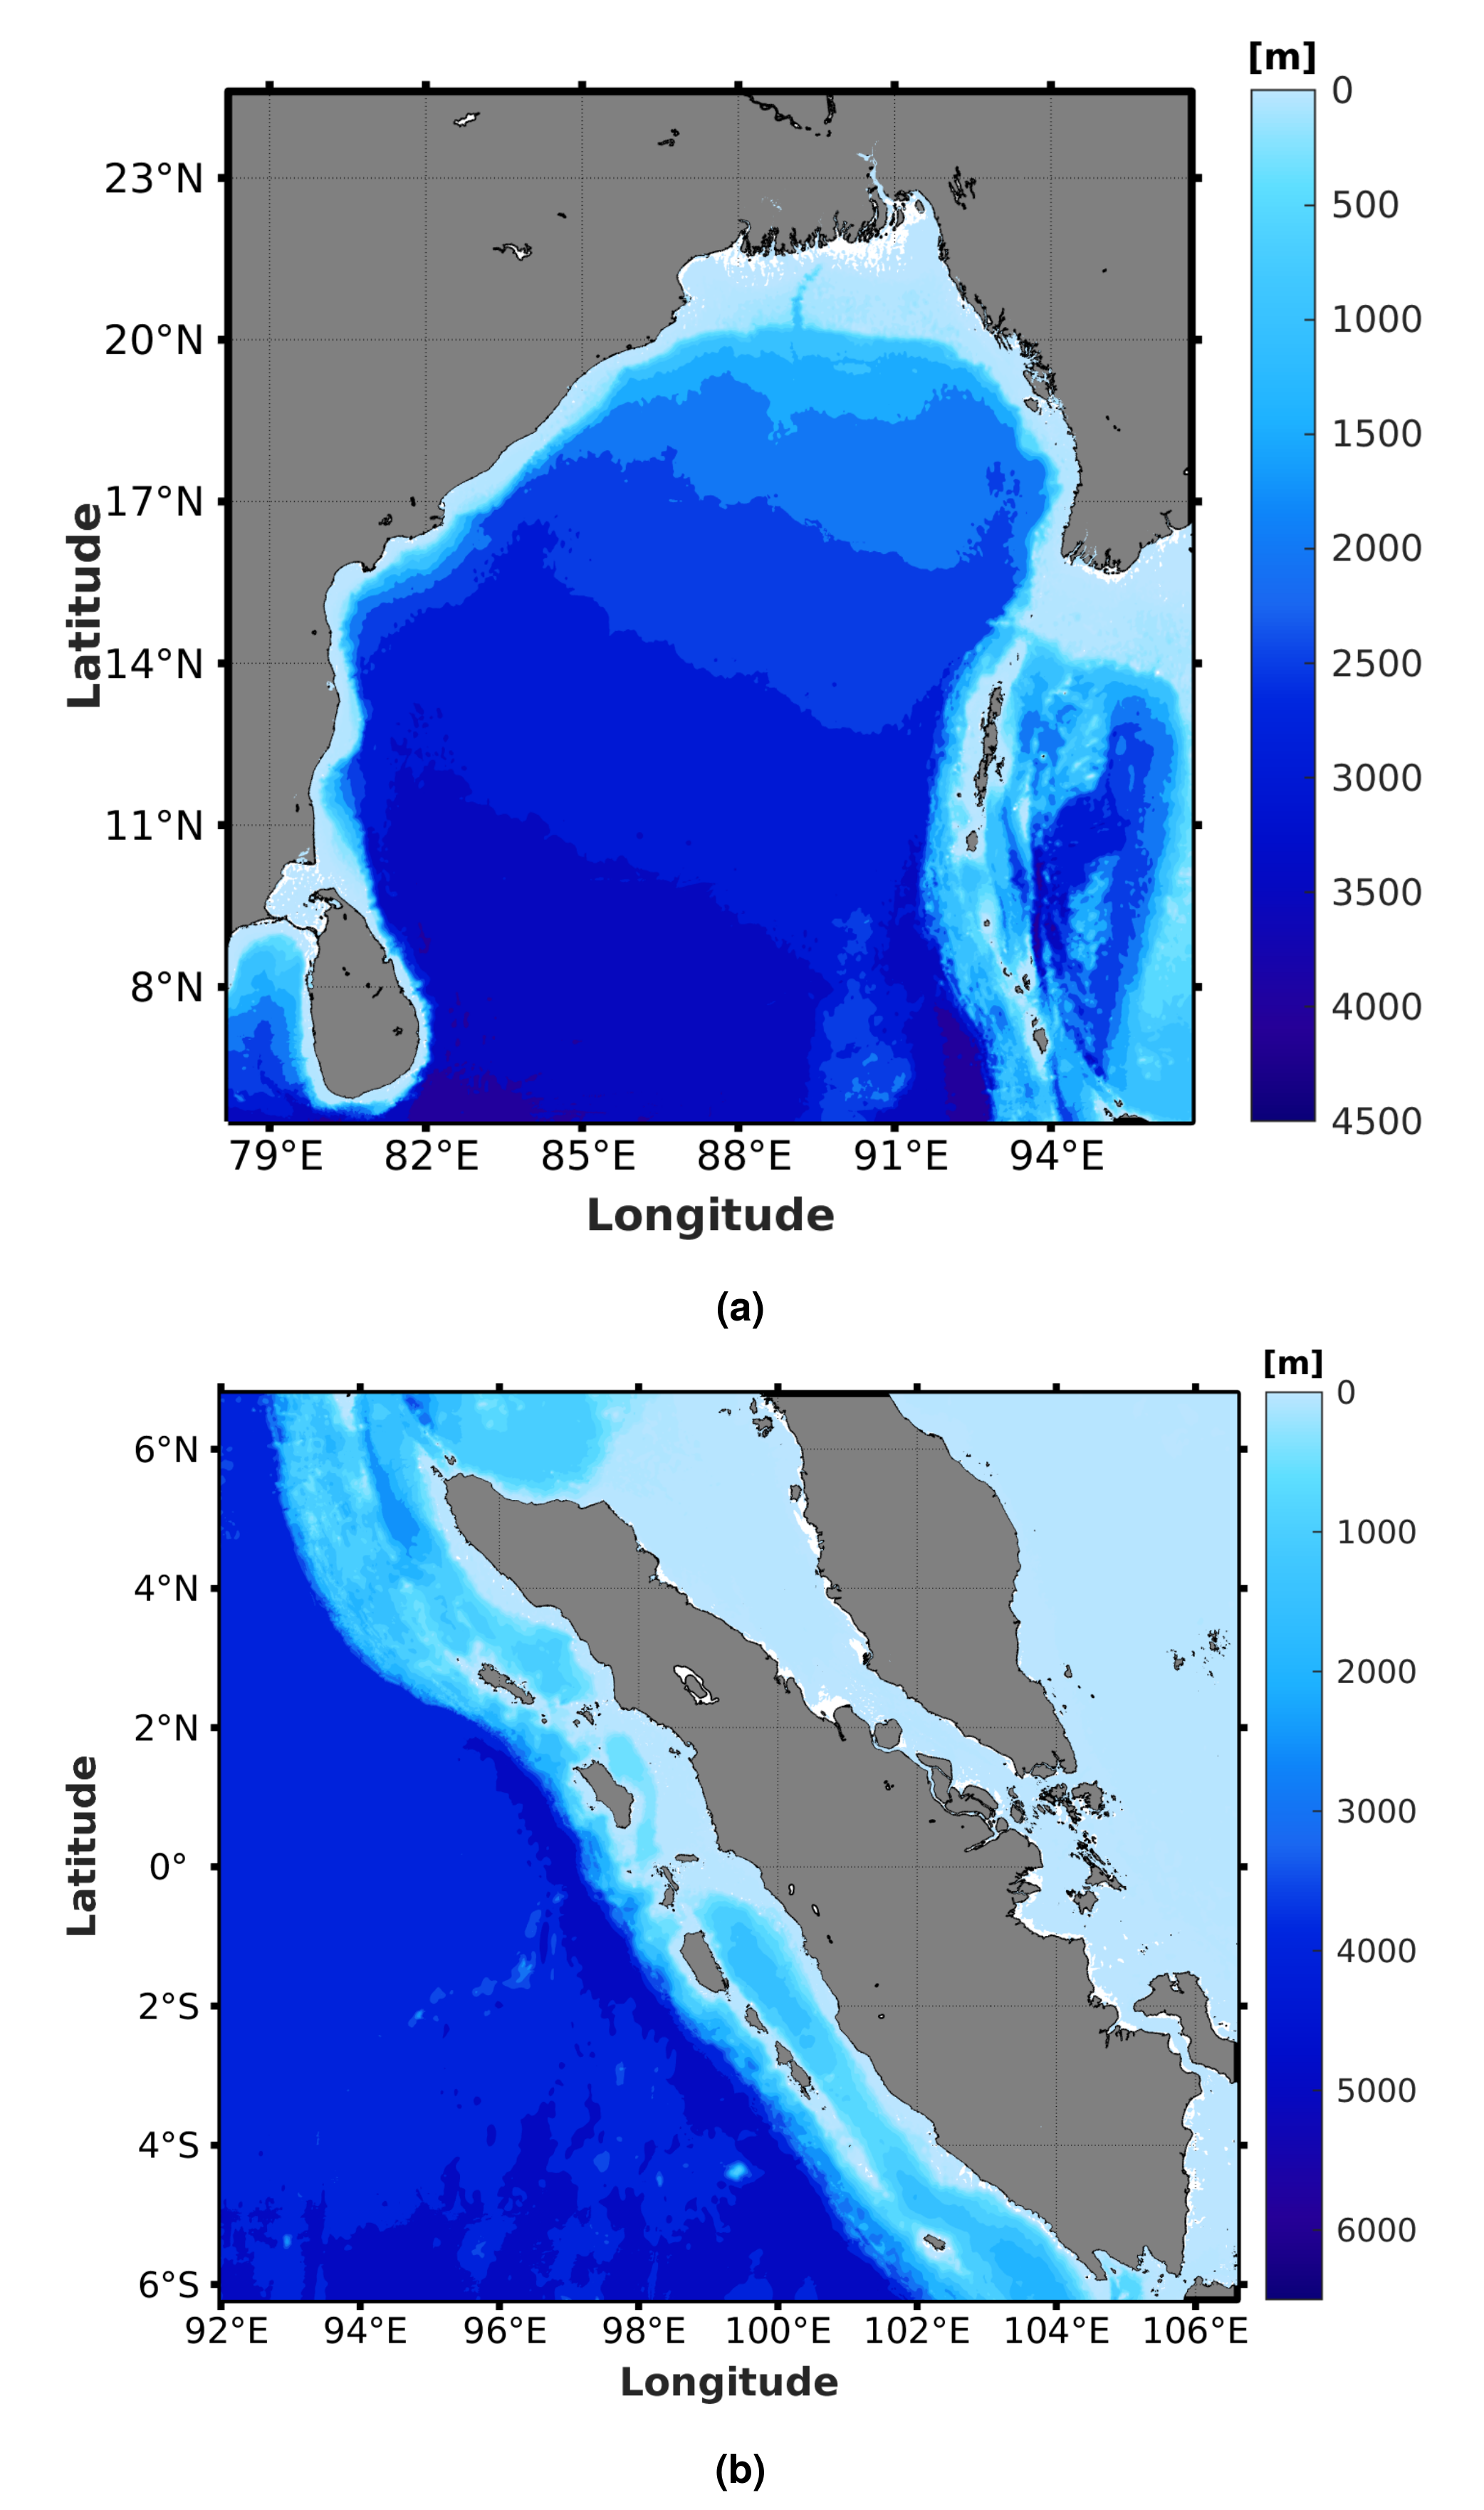
\includegraphics[width=12cm]{contents/Topo}
		\caption{Peta batimetri untuk domain (a) Teluk Benggala (BoB) dan (b) Perairan Aceh, Selat Malaka, Bagian Laut Cina Selatan, dicuplik dari SRTM15+.}
		\label{fig:domain}
	\end{figure}

\end{spacing}
\vspace{-1pc}
\section[Data Penelitian]{Data Penelitian}
\begin{spacing}{1.5}
\vspace{-1pc}
\subsection[Data Oseanografi]{Data Oseanografi}
	Data oseanografi yang digunakan adalah data arus permukaan, serta data temperatur dari model HYCOM (\textit{The Hybrid Coordinate Ocean Model}) dan model NEMO (\textit{Nucleus for European Modeling of the Ocean}) yang merupakan model sirkulasi laut (OGCM) yang menggunakan model numerik tiga dimensi Navier-Stokes.

\subsubsection[HYCOM]{HYCOM}
	Model HYCOM (\textit{HYbrid Coordinate Ocean Model}) (\href{https://www.hycom.org}{https://www.hycom.org}) adalah salah satu model sirkulasi laut (OGCM) yang menggunakan model numerik tiga dimensi Navier-Stokes dengan input data batimetri dari GEBCO (\textit{General Bathymetric Chart of the Oceans}), data asimilasi hidrografi laut dari NCODA (\textit{Navy Coupled Ocean Data Assimilation}) dan komponen meteorologi dari NCEP (\textit{National Centers for Environmental Prediction}) ataupun NAVGEM (\textit{The NAVy Global Environmental Model}) berupa angin, kecepatan, fluks panas, tekanan permukaan laut, presipitasi, temperature, dan kelembapan \shortcite{JosephMetzger2013}. Koordinat vertikal dalam HYCOM adalah isopiknal di lautan terbuka yang terstratifikasi dan memiliki transisi yang mulus dan dinamis serta bergantung terhadap waktu pada medan daerah pesisir yang dangkal dan pada tingkat tekanan tetap di lapisan campuran permukaan atau lautan yang tidak terstratifikasi \shortcite{chassignet2017,Park2013}. 
	\par Data HYCOM yang digunakan adalah data analisis global arus dan temperature tiga dimensi dengan resolusi spasial 5 menit untuk longitude dan 2.5 menit untuk latitude selama 12 bulan (Januari - Desember) tahun 2021 dan dengan ketebalan bervariasi pada bidang vertikal, yaitu 40-lapisan $(k \in [1,40])$:
	\begin{equation*}
		\begin{aligned}
			z_k = \{0.0, 2.0, 4.0, 6.0, 8.0, 10.0, 12.0, 15.0, 20.0, 25.0, 30.0, 35.0, 40.0, 45.0, 50.0, \\
			60.0, 70.0,	80.0, 90.0, 100.0, 125.0, 150.0, 200.0, 250.0, 300.0, 350.0, 400.0, 500.0, 600.0,\\
			700.0, 800.0, 900.0, 1000.0, 1250.0, 1500.0, 2000.0, 2500.0, 3000.0, 4000.0, 5000.0\} (m). \\
		\end{aligned}
	\end{equation*}

\subsubsection[NEMO]{NEMO}
	Model NEMO adalah model komputasi resolusi tinggi yang digunakan untuk kegiatan penelitian dan layanan peramalan dalam oseanografi dan klimatologi, yang dikembangkan secara berkelanjutan sejak 2008 oleh konsorsium Eropa yang terdiri dari 5 institusi (CMCC | CNRS | Mercator Ocean | Met Office | NERC). Hal ini dimaksudkan untuk menjadi alat yang fleksibel untuk mempelajari fenomena fisik dan biogeokimia dalam sirkulasi laut, serta interaksinya dengan komponen sistem iklim Bumi, pada berbagai skala ruang dan waktu \shortcite{madec_gurvan_2022_6334656}. 
	
	Penelitian ini menggunakan data output model NEMO (\href{https://www.nemo-ocean.eu/}{https://www.nemo-ocean.eu/}) untuk data analisis global arus dan temperatur tiga dimensi yang didownload dari website CMEMS (\textit{Copernicus Marine Environment Monitoring Service}) \href{https://resources.marine.copernicus.eu/products}{(https://resources.marine.copernicus.eu/products)} selama 12 bulan (Januari - Desember) tahun 2021.  Dalam analisis penelitian ini, resolusi data output yang digunakan adalah dx = dy = 5 menit pada bidang horizontal dan 50-lapisan $(k \in [1,50])$ dengan ketebalan berbeda pada bidang vertikal:
	\begin{equation*}
		\begin{aligned}
			z_k = \{0.49, 1.54, 2.65, 3.82, 5.08, 6.44, 7.93, 9.57, 11.40, 13.47, 15.82, 18.50, \\
			21.60, 25.21, 29.44, 34.43, 40.34, 47.37, 55.76, 65.81, 77.85, 92.33, 109.73, 130.67, \\
			155.85, 186.12, 222.47, 266.04, 318.13, 380.21, 453.94, 541.089, 643.57, 763.33, \\
			902.34, 1062.44, 1245.29, 1452.25, 1684.28, 1941.89, 2225.08, 2533.33, 2865.70,  \\
			3220.82, 3597.03, 3992.48, 4405.22, 4833.29, 5274.78, 5727.92 \} (m). \\
		\end{aligned}
	\end{equation*}

\subsection[Data Meteorologi]{Data Meteorologi}
	Data meteorologi yang digunakan adalah data reanalysis NCEP/NCAR per 6 jam \href{https://psl.noaa.gov/data/gridded/data.ncep.reanalysis.html}{(https://psl.noaa.gov/data/gridded/data.ncep.reanalysis.html)} selama 20 tahun dari tahun 2002 sampai 2021 untuk 6 parameter yaitu: \textit{2m air temperature, 2m specific humidity, convective precipitation rate, sea level pressure, wind stress U}, dan \textit{wind stress V}.
\subsubsection[2m \textit{Air Temperature}]{2m \textit{Air Temperature}}
	2m \textit{air temperature} atau temperature udara 2m adalah temperature udara yang berada pada 2 meter di atas permukaan (laut atau tanah). Satuan dari temperature udara 2m adalah $^\circ$C.
\subsubsection[2m \textit{Specific Humidity}]{2m \textit{Specific Humidity}}
	 2m \textit{specific humidity} atau kelembaban spesifik 2m mengacu pada berat (jumlah) uap air yang terkandung dalam satuan berat (jumlah) udara yang berada pada 2 meter di atas permukaan (laut atau tanah). Satuan dari temperature udara 2m adalah $kg/kg$.
\subsubsection[\textit{Convective Precipitation Rate}]{\textit{Convective Precipitation Rate}}
	\textit{Convective precipitation rate} atau laju presipitasi konvektif adalah laju presipitasi yang dihasilkan oleh skema konveksi. Presipitasi konvektif terjadi ketika udara naik secara vertikal melalui mekanisme konveksi mandiri (berlangsung secara singkat). Satuan dari laju presipitasi konvektif adalah $kg/m^2s$.
\subsubsection[\textit{Sea Level Pressure}]{\textit{Sea Level Pressure}}
	\textit{Sea level pressure} atau tekanan permukaan laut adalah tekanan atmosfer pada permukaan laut. Satuan dari tekanan permukaan laut adalah $kPa$.
\subsubsection[\textit{Wind Stress}]{\textit{Wind Stress}}
	\textit{Wind stress} atau tekanan angin adalah gaya geser per satuan luas yang diberikan oleh angin yang bertiup di atas permukaan laut. Tekanan angin berupa vektor tekanan angin $U$ dan tekanan angin $V$. Satuan dari tekanan angin adalah $Pa$.
\end{spacing}
\vspace{-0.5pc}
\section[Metode Interpolasi]{Metode Interpolasi}
\begin{spacing}{1.5}
	Metode interpolasi yang digunakan adalah interpolasi linear. Misalkan terdapat fungsi $f$ yang tidak diketahui. Akan dicari nilai titik $P=(x,y)$ dengan menggunakan interpolasi linear. 
	\begin{figure}[H]
		\centering
		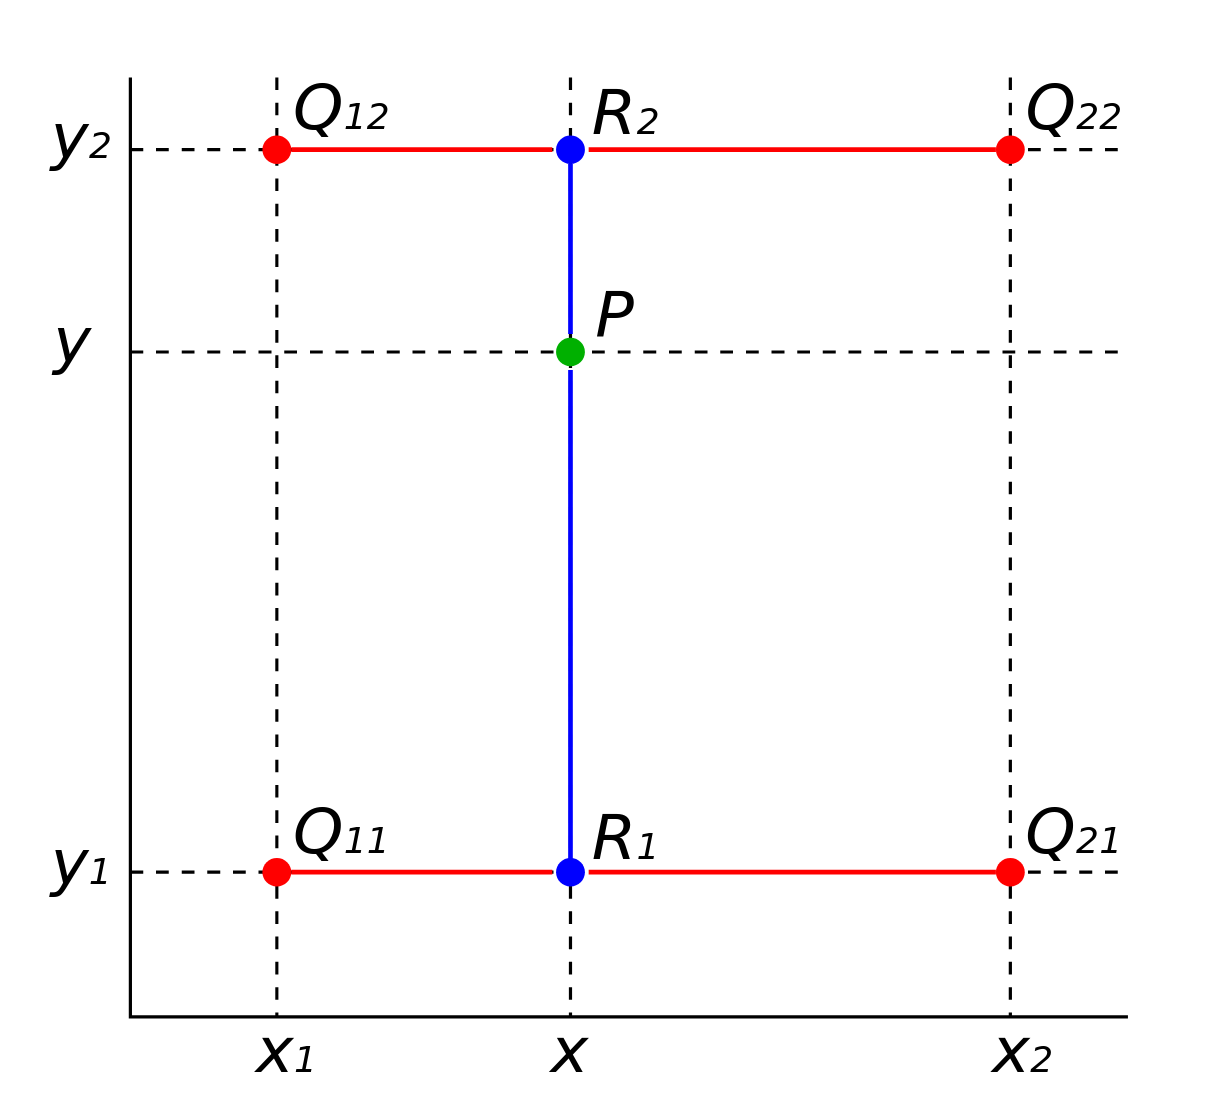
\includegraphics[width=6cm]{contents/BilinearInterpolationV2}
		\caption{Titik-titik yang akan diinterpolasi.} 
		\label{fig:interp}
		\medspace
		\small
		Titik $Q_{11},Q_{12},Q_{21}$ dan $Q_{22}$ (titik merah) adalah titik yang diketahui dan titik $P$ (titik hijau) adalah titik yang akan diinterpolasi.
	\end{figure}
	Asumsikan bahwa nilai 4 titik diketahui, titik $Q_{11}=(x_1,y_1),Q_{12}=(x_1,y_2),Q_{21}=(x_2,y_1)$ dan $Q_{22}=(x_2,y_2)$. Persamaan untuk fungsi interpolasi linear dalam arah sumbu-x diberikan oleh
	\begin{equation*}
		\begin{aligned}
			f(x,y_1)&=\frac{x_2-x}{x_2-x_1}f(Q_{11})+\frac{x-x_1}{x_2-x_1}f(Q_{21}),\\
			f(x,y_2)&=\frac{x_2-x}{x_2-x_1}f(Q_{12})+\frac{x-x_1}{x_2-x_1}f(Q_{22}).
		\end{aligned}
	\end{equation*}
	Interpolasi untuk arah sumbu-y ketika dilanjutkan akan memberikan persamaan yang lengkap sebagai berikut
	\begin{equation*}
		 \resizebox{\textwidth}{!}{% 
			$
		\begin{aligned}
			f(x,y)&=\frac{y_2-y}{y_2-y_1}f(x,y_1)+\frac{y-y_1}{y_2-y_1}f(x,y_2)\\
			&=\frac{y_2-y}{y_2-y_1}\left(\frac{x_2-x}{x_2-x_1}f(Q_{11})+\frac{x-x_1}{x_2-x_1}f(Q_{21})\right)+\frac{y-y_1}{y_2-y_1}\left(\frac{x_2-x}{x_2-x_1}f(Q_{12})+\frac{x-x_1}{x_2-x_1}f(Q_{22})\right)\\
			&=\frac{1}{(x_2-x_1)(y_2-y_1)}(f(Q_{11})(x_2-x)(y_2-y)+f(Q_{21})(x-x_1)(y_2-y)+f(Q_{12})(x_2-x)(y-y_1)\\
			&+f(Q_{22})(x-x_1)(y-y_1))\\
			&=\frac{1}{(x_2-x_1)(y_2-y_1)}[x_2-x \quad x-x_1]\binom{f(Q_{11})\quad f(Q_{12})}{f(Q_{21})\quad f(Q_{22})}\binom{y_2-y}{y-y_1}.%
		\end{aligned}
		$
	}
	\end{equation*}
		Dengan cara yang sama, interpolasi untuk parameter meteorologi dapat dilakukan dengan mengganti nilai $x,y,$ dan $f$ di atas dengan nilai longitude, latitude, dan nilai untuk parameter meteorologi yang bersesuaian.
\end{spacing}	
\vspace{-0.5pc}
\section[Prosedur Penelitian]{Prosedur Penelitian}
\subsection[Penentuan MLD]{Penentuan MLD}
\begin{spacing}{1.5}
	MLD ditentukan dengan menggunakan data temperature HYCOM dari hasil penggambaran \textit{cross-section} pada bagian selatan BoB, di latitude 9$^\circ$C, dan bagian utara BoB, di latitude 19$^\circ$C. \textit{Cross-section} temperature menggunakan kriteria beda hingga, khususnya kriteria nilai \textit{threshold} temperature, $\Delta t=0.1^\circ$C dengan referensi dari permukaan laut \shortcite{Sprintall1999}. Cara yang digunakan untuk mengestimasi ketebalan MLD adalah dengan cara melihat perubahan temperature pada setiap kedalaman. Gambar \textit{cross-section} temperature diplot terlebih dahulu tanpa kontur menggunakan kriteria \textit{threshold} 0.1$^\circ$C untuk menghasilkan gambar dengan warna biru, hijau, dan kuning yang berbeda yang merupakan representasi dari perubahan temperature. Gambar kontur kemudian ditambahkan untuk melihat secara jelas nilai temperature berdasarkan interval 1$^\circ$C. Indikator nilai ketebalan MLD berdasarkan perubahan warna dan temperature yang terjadi pertama kali dari permukaan laut pada gambar.
	
	\begin{figure}[H]
		\centering
		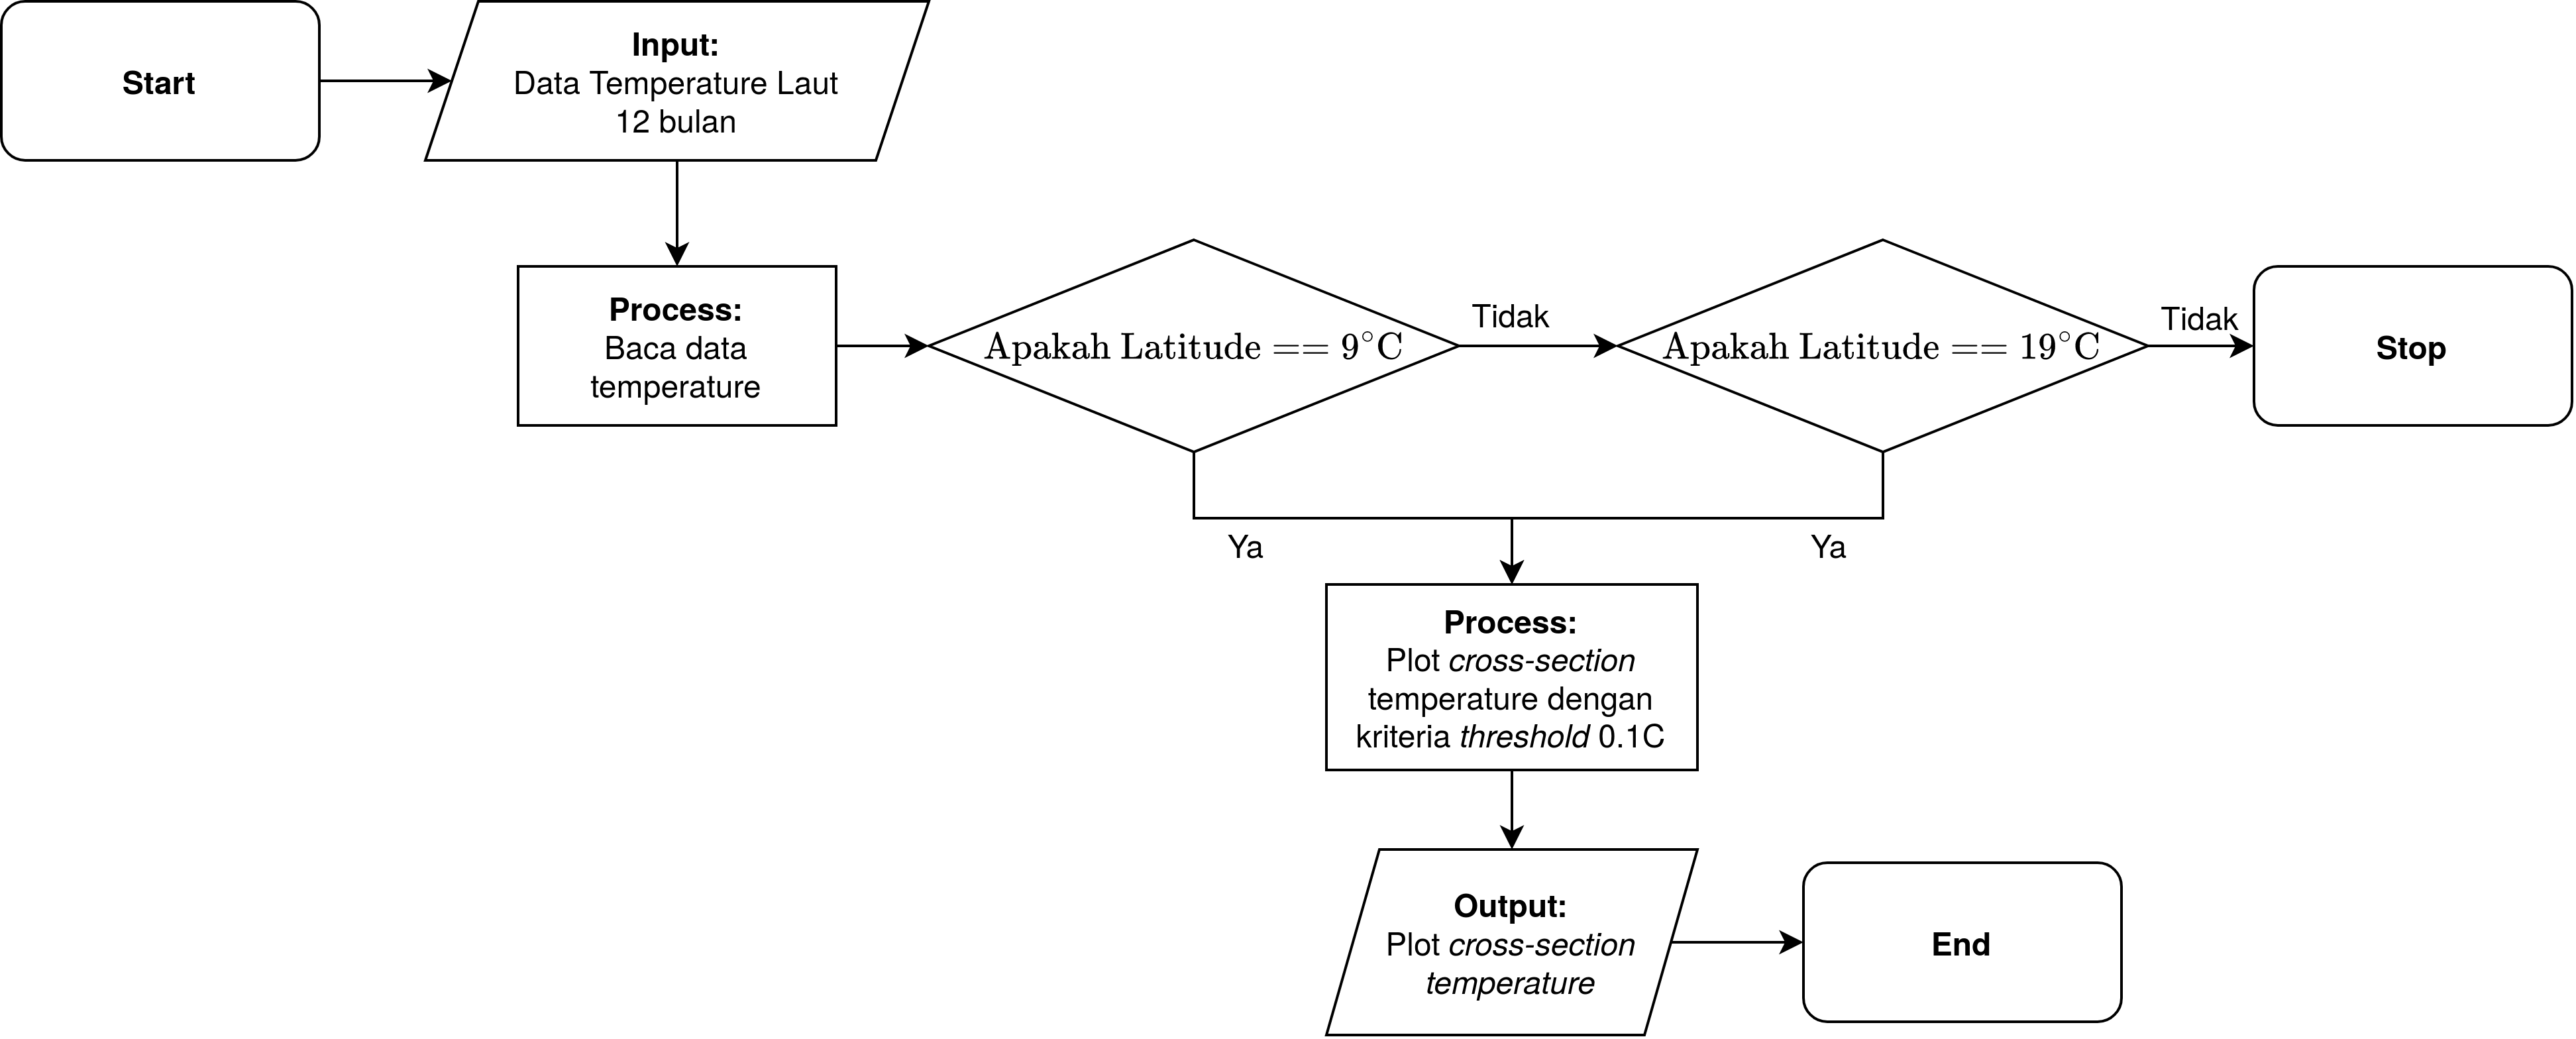
\includegraphics[width=14cm]{contents/Flowchart_1.png}
		\caption{Diagram alir penentuan MLD.}
		\label{fig:flowchart_1}
	\end{figure}
\subsection[Model Iklim (\textit{Seasonal Model})]{Model Iklim (\textit{Seasonal Model})}
	Data meteorologi NCEP/NCAR diinterpolasi dengan menggunakan metode yang telah dijelaskan sebelumnya kemudian dianalisis menggunakan sinyal musiman dengan persamaan sebagai berikut (Haridhi et al., 2016):
	\begin{equation}\label{eq:sm}
		y = \alpha + \beta \sin(2\pi t)+\gamma \cos(2\pi t)
	\end{equation}
	dengan $\alpha$ adalah konstanta pergesaran vertikal, $\beta$ adalah amplitude dari gelombang sinus, $\gamma$ adalah amplitude dari gelombang kosinus, $t$ adalah waktu.
	
	Rumus ini tidak hanya digunakan untuk menjelaskan pola musiman, tetapi rumus ini juga dapat memprediksi parameter dan peristiwa MLD berdasarkan keteraturannya \shortcite{Ikhwan2022}. Pemilihan musim dengan formula ini mempengaruhi kesesuaian musim yang terjadi. Di Laut Andaman dan Selat Malaka, monsun yang terjadi adalah monsun timur laut (NEM) dan monsun barat daya (SWM), sehingga asumsi monsun ini juga dapat terjadi di BoB \shortcite{Rizal2012a}.
	\begin{figure}[H]
		\centering
		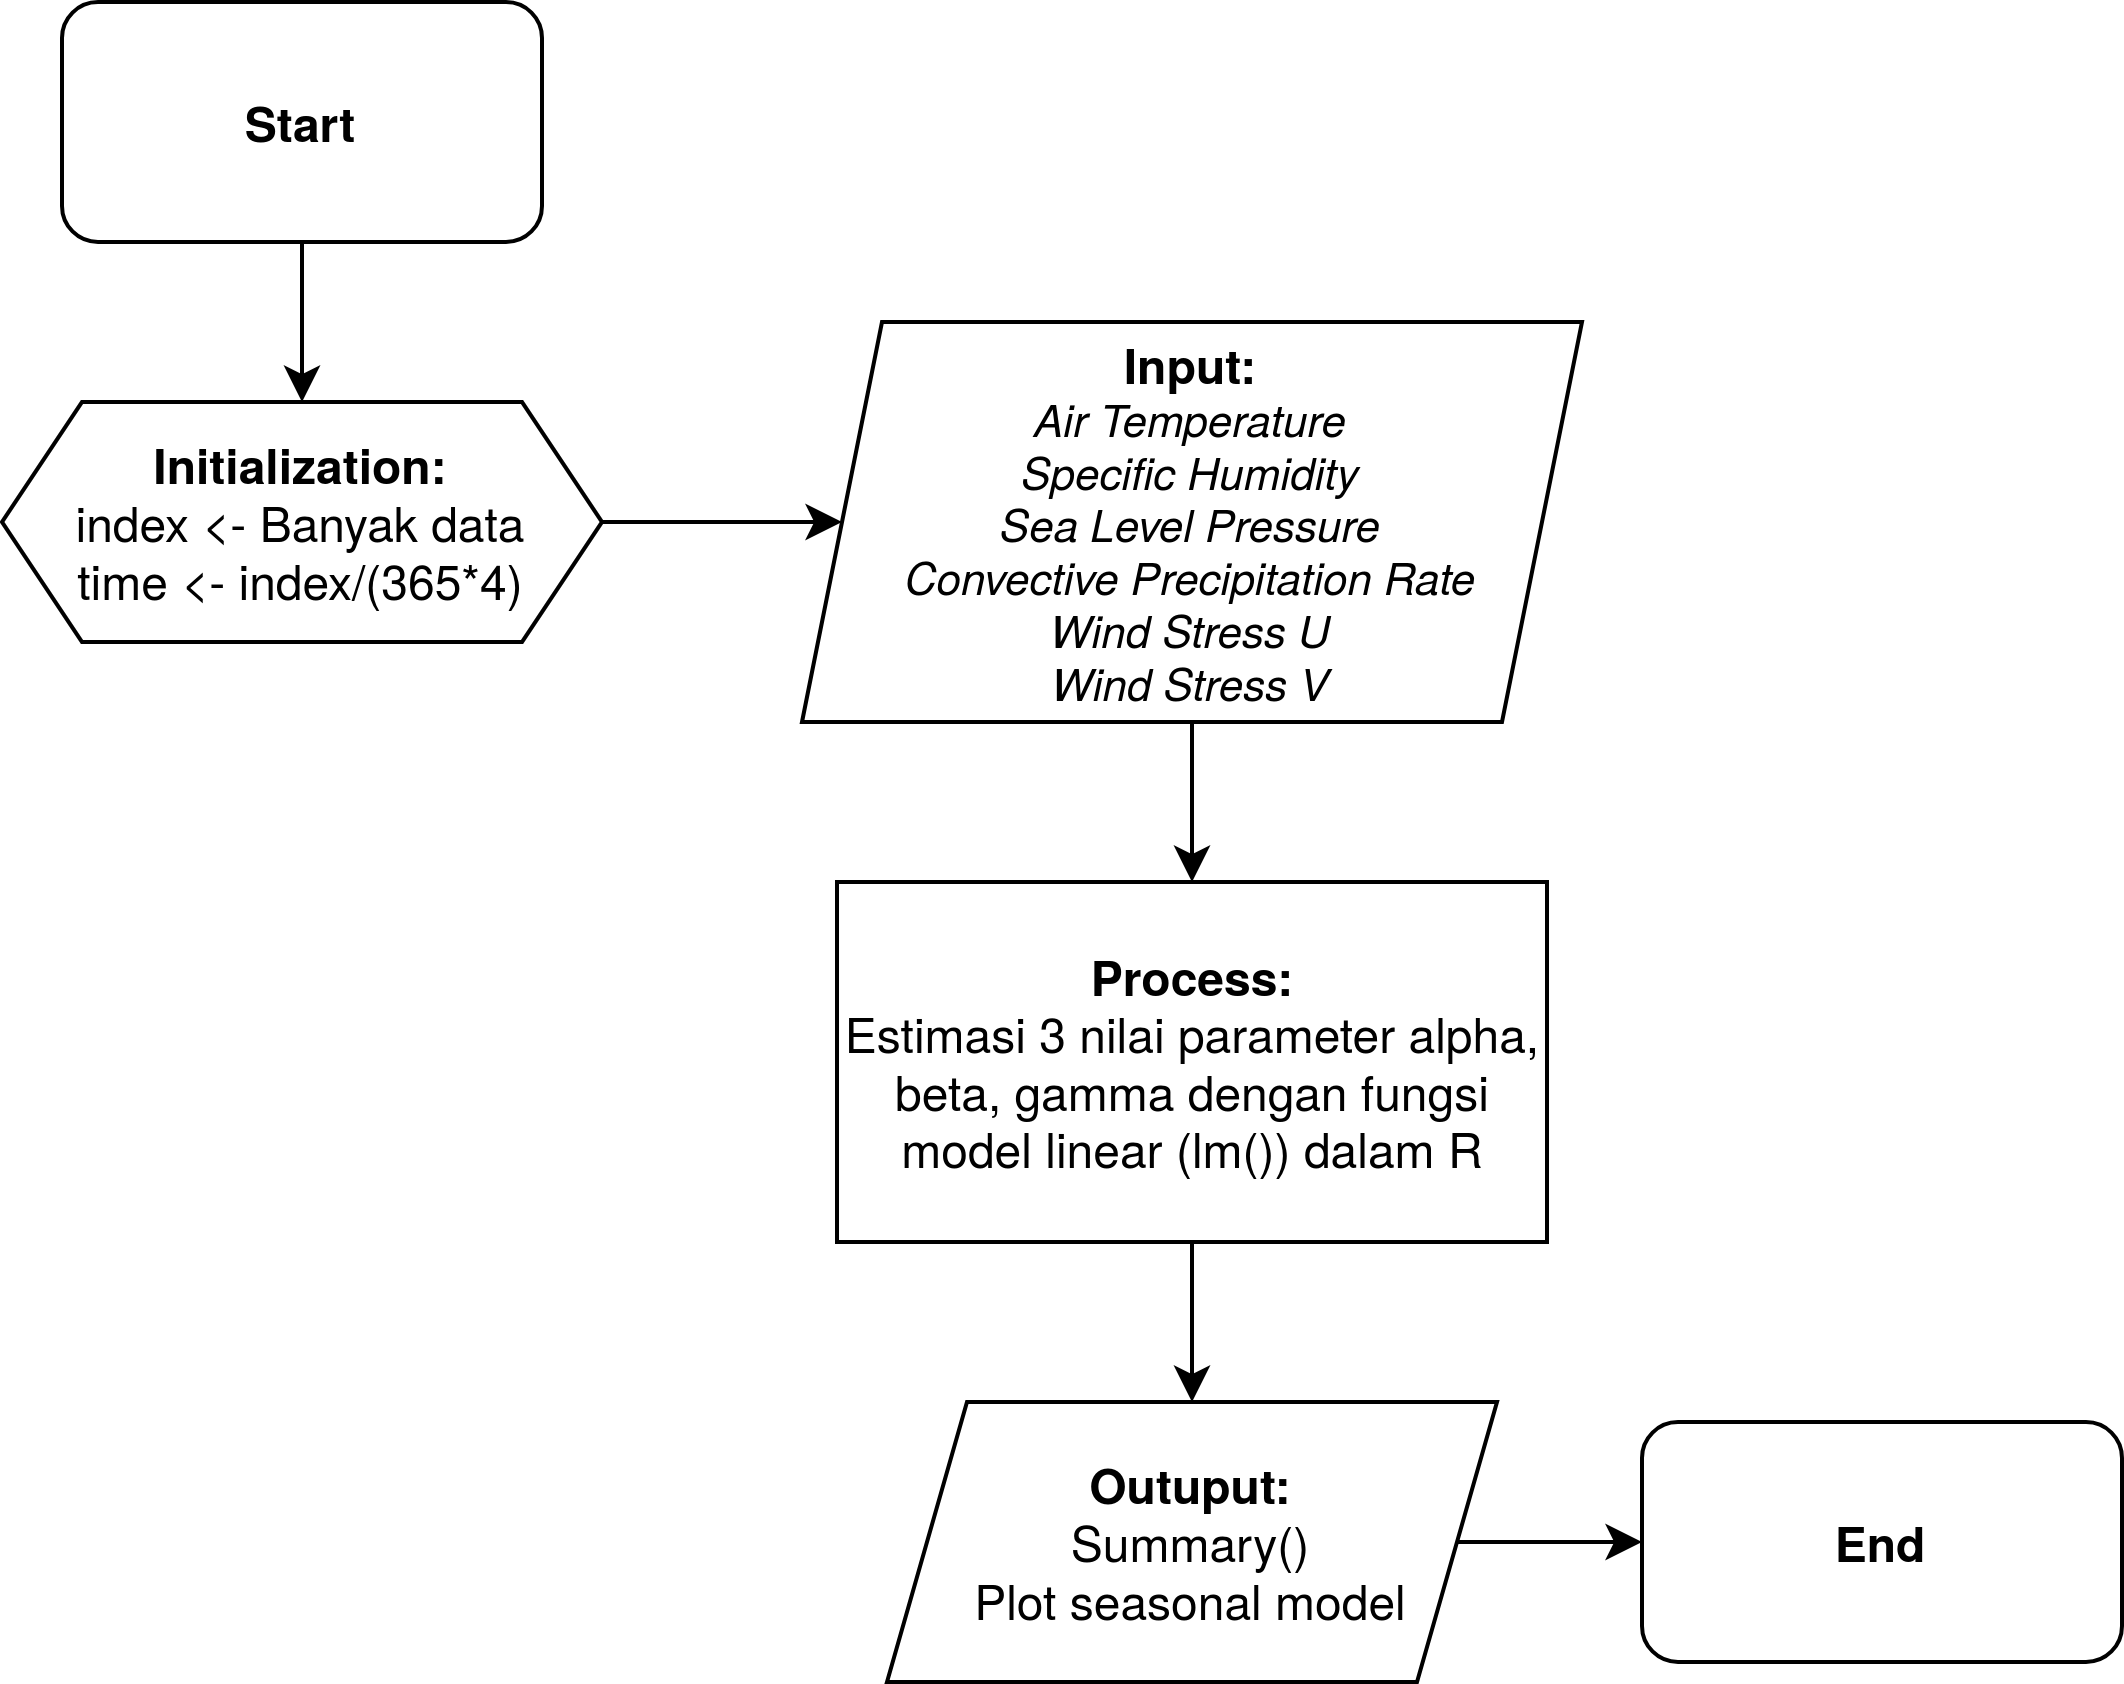
\includegraphics[width=12cm]{contents/Flowchart_2.png}
		\caption{Diagram alir \textit{seasonal model}.}
		\label{fig:flowchart_2}
	\end{figure}
\subsection[Alur Penelitian]{Alur Penelitian}
	\begin{figure}[H]
		\centering
		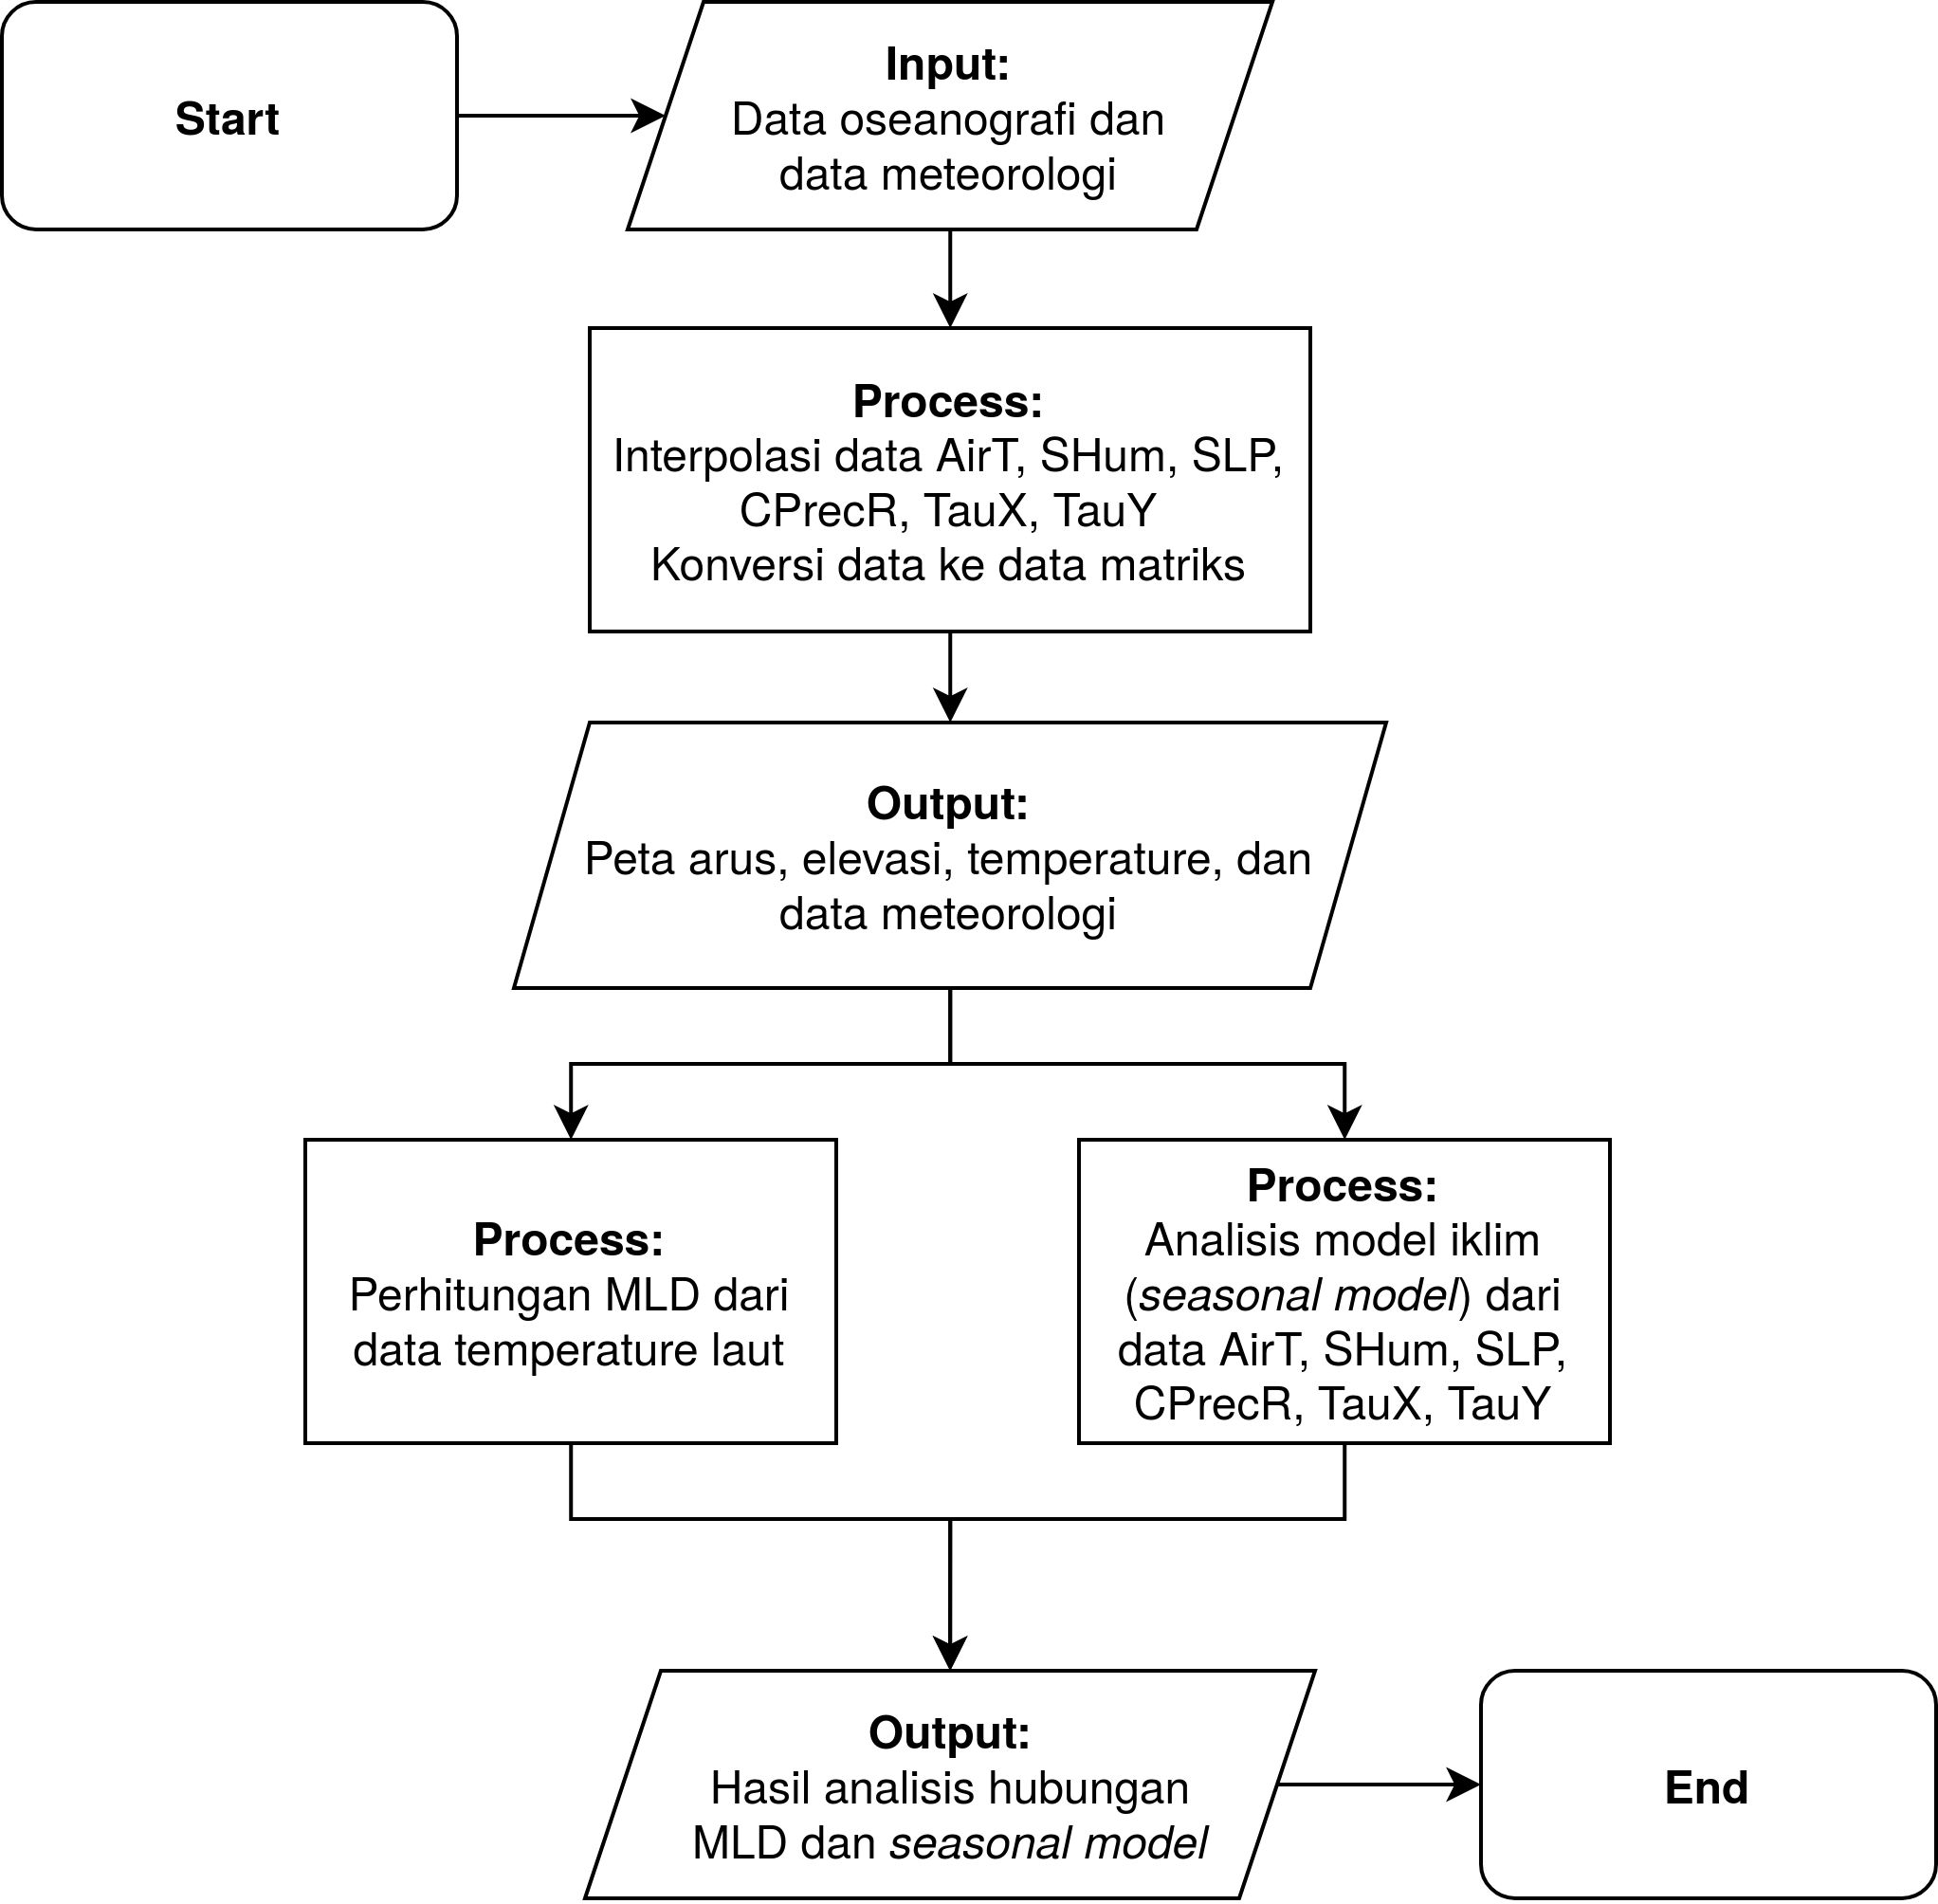
\includegraphics[width=10cm]{contents/Flowchart_Diagram.png}
		\caption{Diagram alir penelitian}
		\label{fig:flowchart}
	\end{figure}
	Prosedur penelitian mengikuti diagram alir pada Gambar \ref{fig:flowchart}. Data-data terkait penelitian didownload terlebih dahulu kemudian diinterpolasi untuk memenuhi data yang kosong serta untuk memperoleh resolusi spasial yang lebih detail. Selanjutnya data hasil interpolasi kemudian dibaca dan di konversi ke dalam data matriks pada MATLAB. Hasilnya adalah peta arus, elevasi, temperature, dan data meteorologi. Peta temperature kemudian diobservasi untuk menentukan kedalaman lapisan campuran selama 12 bulan. Sebagai verifikasi atas observasi kedalaman lapisan campuran, akan dilakukan analisis model iklim terhadap data meteorologi (\textit{2m air temperature, 2m specific humidity, convective precipitation rate, sea level pressure, wind stress U}, dan \textit{wind stress V}) selama 22 tahun dari tahun 2002 sampai 2021.
\end{spacing}
\vspace{-0.5pc}

\section[Metode Analisis Korelasi]{Metode Analisis Korelasi}
\begin{spacing}{1.5}
	Penelitian ini menganalisis tentang hubungan antara Chl-a - SST, Chl-a - SSS dan SST - SSS dengan menggunakan analisis korelasi Pearson (penelitian ini menggunakan data populasi agar kesimpulan yang diperoleh lebih akurat). Tabel Uji hipotesis statistic t (t-statistic or t-value) dan tabel analysis of variance (ANOVA) juga disajikan untuk menguji hipotesis penelitian mengenai pengaruh dari masing-masing variabel dan untuk mengetahui apakah ada perbedaan yang signifikan antara rata-rata hitung (mean) untuk variable yang diamati. Persamaan korelasi dan koefisien korelasi yang digunakan adalah \shortcite{Haditiar2019,Xu2016},
	\begin{equation}
		\begin{aligned}
			y &= a+rx\\
			r &= \frac{\sum (x_i - \bar{x})(y_i - \bar{y})}{\sqrt{\sum (x_i-\bar{x})^2\sum (y_i-\bar{y})^2}}
		\end{aligned}
	\end{equation}

	Dengan $\alpha$ adalah konstanta titik potong sumbu-$y$, $r$ adalah kemiringan dari garis regresi (koefisien regresi), $x_i, y_i$ adalah variable yang ingin dibandingkan (dapat berupa Chl-a, SST, dan SSS) dimana $i$ adalah indeks kordinat latitude-longitude yang bersesuaian, $\bar{x},\bar{y}$ adalah rata-rata untuk data populasi. Persamaan untuk RMSE adalah,
	
	\begin{equation}
		\begin{aligned}
			\text{RMSE}=\sqrt{\frac{1}{N}\sum_{i=0}^{N}(x_i-y_i)^2}.
		\end{aligned}
	\end{equation}
	
	Persamaan untuk t-statistik adalah,
	
	\begin{equation}
		\begin{aligned}
			t=\frac{r_{xy}\sqrt{n-2}}{1-r^2_{xy}}
		\end{aligned}
	\end{equation}
	
	Penarikan kesimpulan untuk t-statistik dalam hal ini adalah apabila $\|t\|\geq t_{\text{tabel}}$ dengan ($\alpha=5\%$) maka ada korelasi antara $x$ dan $y$.
\end{spacing}
\vspace{-0.5pc}

\section[Metode Analisis Hubungan \textit{Eddies} dan SSH]{Metode Analisis Hubungan \textit{Eddies} dan SSH}
\begin{spacing}{1.5}
	Hubungan antara eddies, SSH, dan SST di teliti di Samudera Hindia pada bulan April 2020 dengan menganalisis variable SSH dan arus permukaan bersama dengan data angin untuk mendeteksi lokasi mana saja yang terjadi pusaran serta mengonfirmasi hasil yang diperoleh dengan menggunakan data SST. 
\end{spacing}
\vspace{-0.5pc}
%\section[Jadwal Penelitian]{Jadwal Penelitian}
%\begin{spacing}{1.5}
%	Jadwal penelitian ditargetkan paling lama 7 bulan dengan rincian kegiatan disusun berdasarkan tabel berikut:
%% Please add the following required packages to your document preamble:
%% \usepackage{multirow}
%	\begin{table}[htp]
%		\centering
%		\caption{Rencana jadwal pelaksanaan penelitian}
%		\label{table:jadwal}
%		\begin{tabular}{|c|c|ccccccc|}
%			\hline
%			\multirow{2}{*}{No.} & \multirow{2}{*}{Kegiatan} & \multicolumn{7}{c|}{Bulan}                                                                                                                            \\ \cline{3-9} 
%			&                   & \multicolumn{1}{c|}{8} & \multicolumn{1}{c|}{9} & \multicolumn{1}{c|}{10} & \multicolumn{1}{c|}{11} & \multicolumn{1}{c|}{12} & \multicolumn{1}{c|}{1} &  2 \\ \hline 1
%			& Studi literatur   & \multicolumn{1}{c|}{X} & \multicolumn{1}{c|}{X} & \multicolumn{1}{c|}{} & \multicolumn{1}{c|}{} & \multicolumn{1}{c|}{} & \multicolumn{1}{c|}{} &  \\ \hline 2
%			& Seminar proposal    & \multicolumn{1}{c|}{X} & \multicolumn{1}{c|}{} & \multicolumn{1}{c|}{} & \multicolumn{1}{c|}{} & \multicolumn{1}{c|}{} & \multicolumn{1}{c|}{} &  \\ \hline 3
%			& Pengumpulan data    & \multicolumn{1}{c|}{} & \multicolumn{1}{c|}{X} & \multicolumn{1}{c|}{} & \multicolumn{1}{c|}{} & \multicolumn{1}{c|}{} & \multicolumn{1}{c|}{} &  \\ \hline 4
%			& Hasil dan analisis  & \multicolumn{1}{c|}{} & \multicolumn{1}{c|}{} & \multicolumn{1}{c|}{X} & \multicolumn{1}{c|}{X} & \multicolumn{1}{c|}{} & \multicolumn{1}{c|}{} &  \\ \hline 5
%			& Seminar hasil       & \multicolumn{1}{c|}{} & \multicolumn{1}{c|}{} & \multicolumn{1}{c|}{} & \multicolumn{1}{c|}{} & \multicolumn{1}{c|}{X} & \multicolumn{1}{c|}{} &  \\ \hline 6
%			& Ujian sidang        & \multicolumn{1}{c|}{} & \multicolumn{1}{c|}{} & \multicolumn{1}{c|}{} & \multicolumn{1}{c|}{} & \multicolumn{1}{c|}{} & \multicolumn{1}{c|}{X} &  \\ \hline 7
%			& Publikasi           & \multicolumn{1}{c|}{} & \multicolumn{1}{c|}{} & \multicolumn{1}{c|}{} & \multicolumn{1}{c|}{} & \multicolumn{1}{c|}{} & \multicolumn{1}{c|}{X} & X  \\ \hline 
%		\end{tabular}
%	\end{table}

%\end{spacing}
%\vspace{-0.1pc}